\documentclass{beamer}

\usetheme{CambridgeUS}
\usepackage{amsmath}
\providecommand{\pr}[1]{\ensuremath{\Pr\left(#1\right)}}
\providecommand{\cdf}[2]{\ensuremath{\text{F}_{#1}\left(#2\right)}}

\title{Assignment-3} 
\author{Aniket Satpute (CS21BTECH11056)}
\date{\today}
\logo{\large \LaTeX{}}


\begin{document}

\begin{frame}
    \titlepage 
\end{frame}

\logo{}



\section{Problem}
\begin{frame}{Problem Statement}

\textbf{(NCERT Class 12, Exercise 13.5 Q9 )} On a multiple choice examination with three possible answers for each of the five questions, what is the probability that a candidate would get four or more correct answers just by guessing ?

\end{frame}


\section{Solution}

\begin{frame}{Solution}
\begin{block}{Random Variables}
\begin{enumerate}
\item $X_i$: Bernoulli random variables with parameter $p, 1 \leq i \leq 5$
\item $Y$: Binomial random variable given by $Y = \sum_{i = 1}^{i = 5}X_i$
\end{enumerate}
\end{block}
\begin{exampleblock}{Moment Generating Function of $X_i$ and $Y$}
\begin{align}
M_Z(X_i) &= \sum_{k = -\infty}^{k = \infty}z^{-k}P_X(k) \\
&= P_X(0) + z^{-1}P_X(1) = (1 - p) + pz^{-1} \\
\end{align}
\end{exampleblock}
\end{frame} 

\begin{frame}

\begin{exampleblock}{Moment Generating Function of $Y$}
\begin{align}
M_Y(Z) &= E(Z^{-Y}) = E(Z^{-\sum_{i = 1}^{i = 5}X_i}) \\
&= \prod_{i = 1}^{i = 5}E(Z^{-X_i}) \\		
&= [(1 - p) + pz^{-1}]^5 \\
&= \sum_{k = 0}^{k = 5}z^{-k}(\binom{5}{k}(1 - p)^{5 - k}p^k)		
\end{align}
\end{exampleblock}
\begin{alertblock}{PMF of Y}
\begin{align}
\pr{Y = k} = 
\begin{cases}
\binom{5}{k}(1 - p)^{5 - k}p^k, & 0 \leq k \leq 5 \\
0, & \textrm{otherwise}
\end{cases}		
\end{align}
\end{alertblock}
	
\end{frame}

\begin{frame}

\begin{alertblock}{CDF of Y}
\begin{align}
\cdf{Y}{k} = \sum_{i = -\infty}^{i = k}\pr{Y = i} =
\begin{cases}
0, & k < 0 \\
\sum_{K = 0}^{K = k}\binom{5}{K}(1 - p)^{5 - K}p^K, & 0 \leq k < 5 \\
1, & k \geq 5
\end{cases}		
\end{align}
\end{alertblock}
\begin{alertblock}{Problem parameters}
Given:
\begin{enumerate}
\item $p = \frac{2}{3}$
\end{enumerate}   
\end{alertblock}
    
\end{frame}


\begin{frame}{Solution}
\begin{align}
\cdf{Y}{1} &= \sum_{i = 0}^{i = 1}\binom{5}{i}(1 - \frac{2}{3})^{10 - i}(\frac{2}{3})^i \\
&= (\frac{1}{3})^{5} + 5(\frac{1}{3})^4(\frac{2}{3})\\
&= \frac{11}{243}
\end{align}
\\
Probability is $\frac{11}{243}$
\end{frame}

\begin{frame}{PMF}

\begin{figure}[h]
\centering
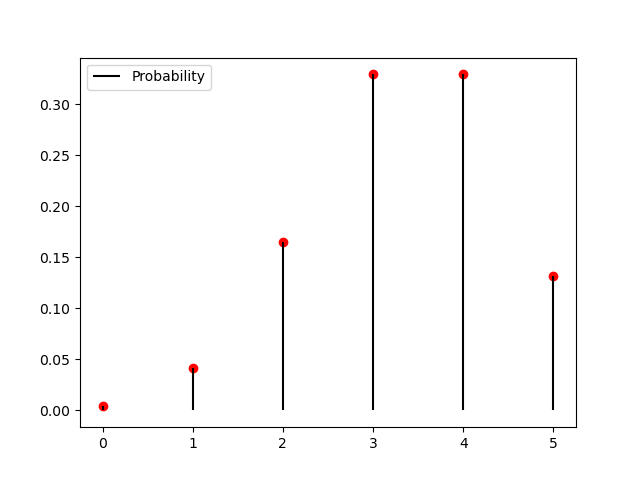
\includegraphics[width=8cm]{PMF.png}
\label{Fig2}
\end{figure}

\end{frame}

\begin{frame}{CDF}

\begin{figure}[h]
\centering
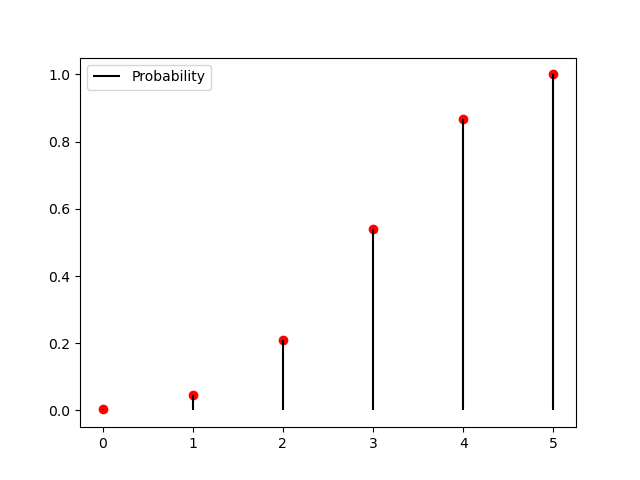
\includegraphics[width=8cm]{CDF.png}
\label{Fig1}
\end{figure}

\end{frame}






\end{document}
